\documentclass[dvipdfmx,autodetect-engine,titlepage]{jsarticle}
\usepackage[dvipdfm]{graphicx}
\usepackage{ascmac}
\usepackage{fancybox}
\usepackage{listings}
\usepackage{plistings}
\usepackage{itembkbx}
\usepackage{amsmath}
\usepackage{svg}
\usepackage{url}
\usepackage{graphics}
\usepackage{listings,jvlisting}

\textheight=23cm
\renewcommand{\figurename}{図}
\renewcommand{\tablename}{表}
\newenvironment{code}
{\vspace{0.5zw}\VerbatimEnvironment  
\begin{screen} 
\baselineskip=1.0\normalbaselineskip
 \begin{Verbatim}}
{\end{Verbatim}
\baselineskip=\normalbaselineskip
 \end{screen}\vspace{0.5zw}} 

\title{情報理工学部 SNコース 3回\\
アプリケーション脆弱性実習レポート\\}
\author{2600200443-6\\Yamashita Kyohei\\山下 恭平}
\date{May 30 2022}

\begin{document}

\maketitle

\section{問1}

\subsection{AchiverSample.zipの展開}

AchiverSample.zipを脆弱アーカイブソフトを用いて展開したところ、
特に異常なくデスクトップに展開することができた。その様子を以下の図1,2に
示す。

\begin{figure}[h]
  \centering
  \begin{minipage}[b]{0.45\linewidth}
  \begin{center}
    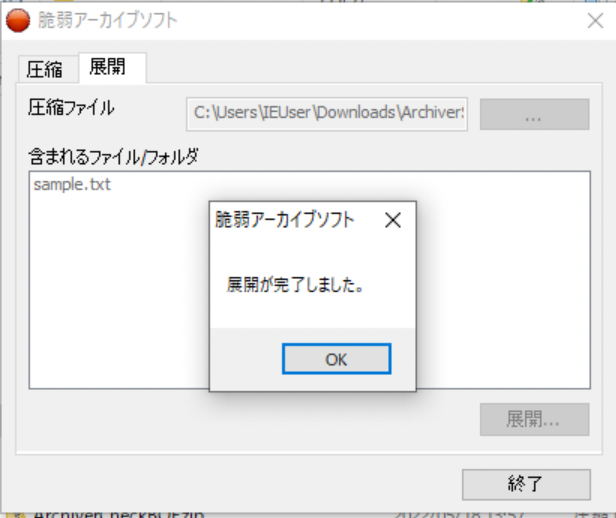
\includegraphics[keepaspectratio,scale=0.65]{pic1-1.png}
    \end{center}
    \caption{}
  \end{minipage}
  \begin{minipage}[b]{0.45\linewidth}
  \begin{center}
    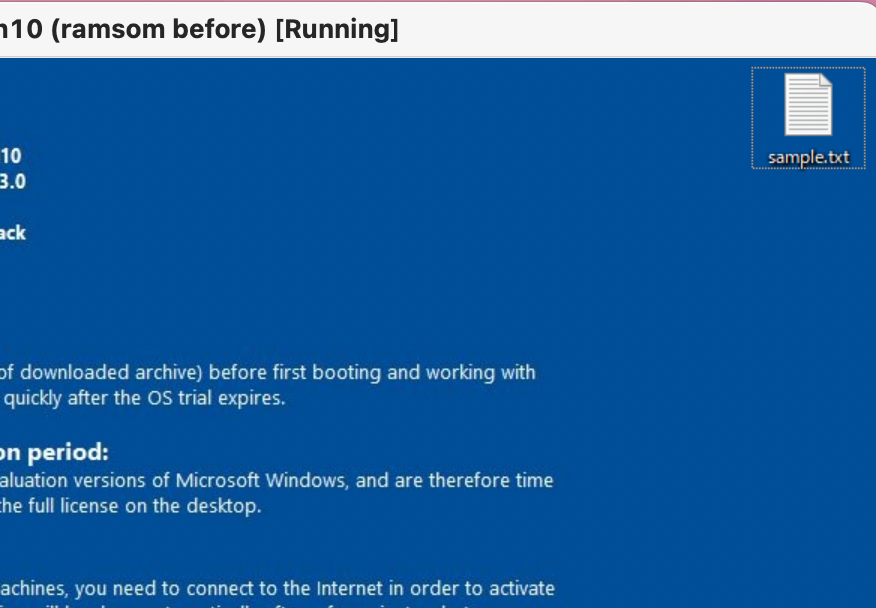
\includegraphics[keepaspectratio,scale=0.55]{pic1-2.png}
    \end{center}
    \caption{}
  \end{minipage}
\end{figure}

\subsection{AchiverCheckBOF.zipの展開}

AchiverCheckBOF.zipを脆弱アーカイブソフトを用いて展開したところ、ソフトが
異常終了を起こし、展開できなかった。その様子を以下の図3に示す。

\begin{figure}[h]
  \centering
  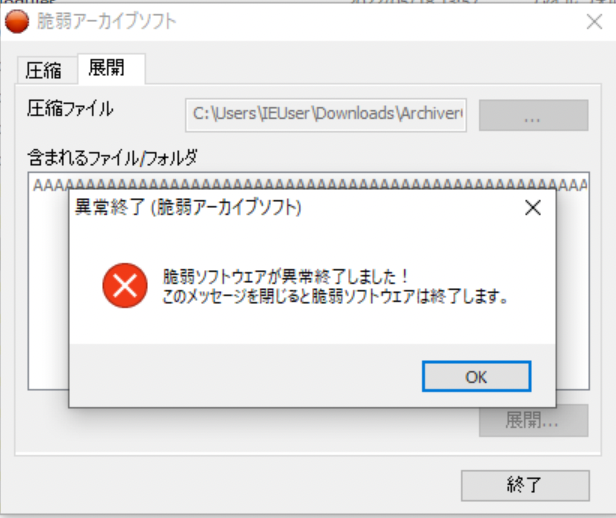
\includegraphics[scale=0.8]{pic2.png}
  \caption{}
\end{figure}

\section{問2}

「AchiverAttackBOF.zip」を展開すると、「AchiverCheckBOF.zip」を展開し
た時と同様に、ダイアログが表示されて、プログラムが終了した。しかし、表示されるダイア
ログは、アプリケーションが強制終了されたことにより表示されたのではなく、オーバーフロー
により、攻撃コードを埋め込まれたことにより表示されている。つまり、今回は展開する
ファイルにダイアログを表示するコードが埋め込まれていたことがわかる。次の図4,5に
それぞれのファイルを展開したときの様子を示す。

\begin{figure}[h]
  \centering
  \begin{minipage}[b]{0.45\linewidth}
  \begin{center}
    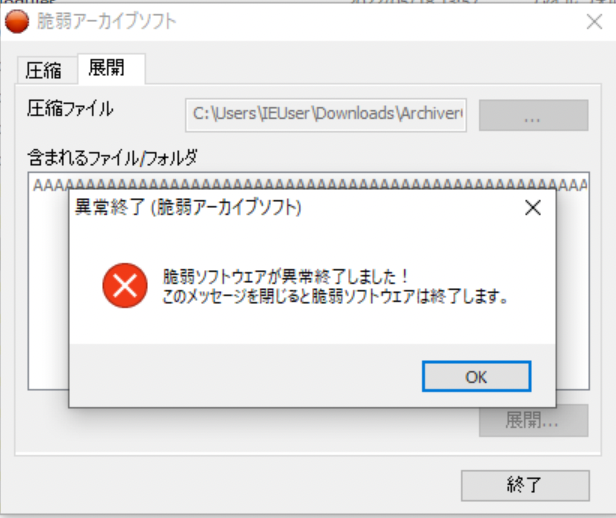
\includegraphics[keepaspectratio,scale=0.6]{pic2.png}
    \end{center}
    \caption{AchiverCheckBOF.zip}
  \end{minipage}
  \begin{minipage}[b]{0.45\linewidth}
  \begin{center}
    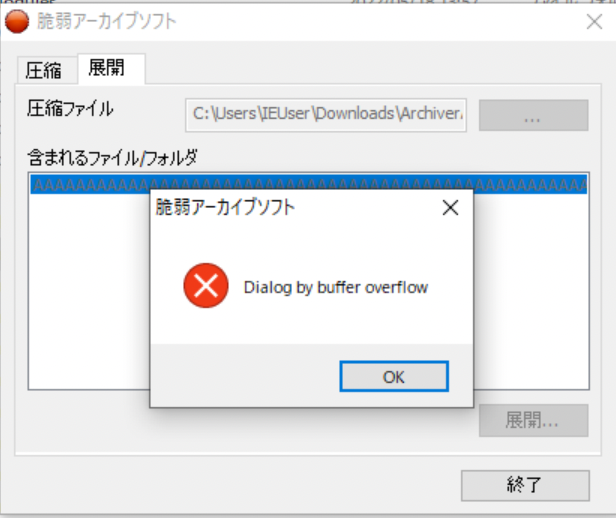
\includegraphics[keepaspectratio,scale=0.6]{pic3.png}
    \end{center}
    \caption{AchiverAttackBOF.zip}
  \end{minipage}
\end{figure}

\subsection{バッファオーバーフローが起きた際に起こる不具合の理由}

\subsubsection*{プログラムの異常終了}
オーバーフローにより、スタック領域に格納されている、呼び出される関数のアドレスや
、関数からの戻りアドレスが書き換えられてしまうことで、プログラムが動作する上で、
必要な関数等にアクセスできなくなるので、プログラムが異常終了する。\\
つまり、オーバフローを起こしても、元から格納されていたものと同一の内容で書き換えれば、
プログラムは正常に動作すると考えられる。

\subsubsection*{プログラムの表示、変数値のバグ}
オーバフローにより、元々設定されていた文字列などの情報も書き換えてしまうから。

\subsection{スッタクオーバーフローを用いた攻撃方法と、その動作原理}
オーバーフローにより、関数の戻りアドレスを書き換えることで、任意のアドレスに
ジャンプすることができる。この時、ジャンプ先のアドレスに対してもオーバーフロー
を利用し、任意の機械語を埋め込んでおくことで、攻撃者の意図した動作をさせることが
できる。

\subsection{フォーマット文字列攻撃における「\%n」の危険性}
\%n書式は、その書式の直前の文字数を格納することができる書式である。\\
例えば、printf("HELLO\%n", \&n);と書き込むとnには5が格納される。よって、
攻撃者は、任意の値をオーバーフローなどを起こさずに、書き込むことが可能であ
る。さらに、「\%(任意の数字)\$n」と入力することで、スタック上の任意の位置を
指定し、任意のコードを埋め込むことが可能である。

\section{問4}

「AchiverCheckIOF.zip」を展開すると、プログラムが異常終了した。
これは、脆弱アプリケーションが圧縮ファイルを展開する際の演算において、
整数オーバーフローが発生し、プログラムが正常に動作しなくなったことで
異常終了したと考えられる。次に、「AchiverAttackIOF.zip」を展開したところ
、プログラムが停止したが、表示されるダイアログは脆弱アプリケーションのものとは
別であることから、整数オーバーフローを利用して、攻撃者が埋め込んだコードが
実行されたと考えられる。



\begin{figure}[h]
  \centering
  \begin{minipage}[b]{0.45\linewidth}
  \begin{center}
    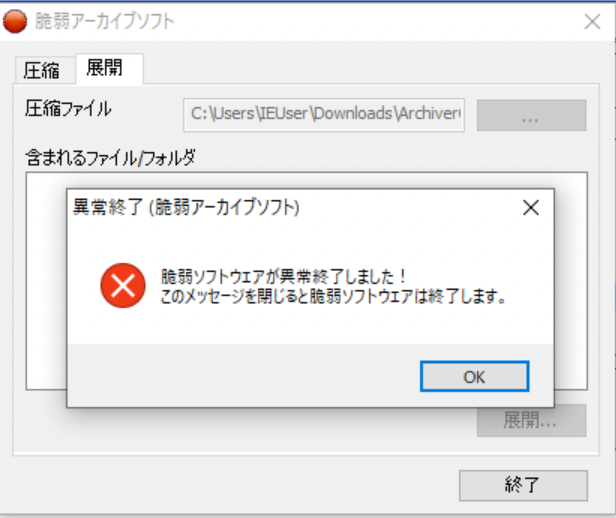
\includegraphics[keepaspectratio,scale=0.6]{pic4.png}
    \end{center}
    \caption{AchiverCheckIOF.zip}
  \end{minipage}
  \begin{minipage}[b]{0.45\linewidth}
  \begin{center}
    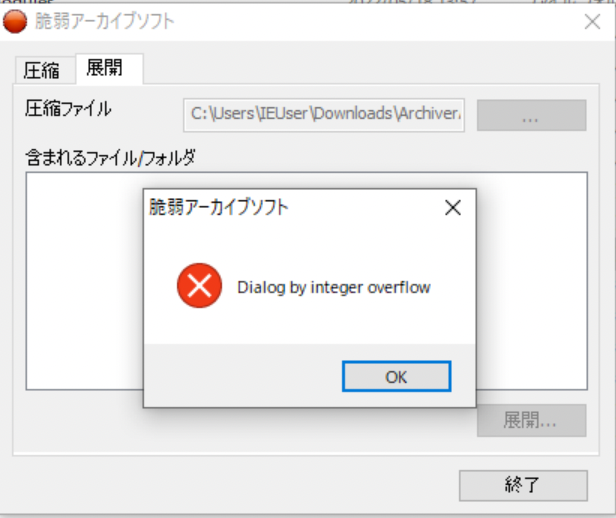
\includegraphics[keepaspectratio,scale=0.6]{pic5.png}
    \end{center}
    \caption{AchiverAttackIOF.zip}
  \end{minipage}
\end{figure}



\end{document}

